\section{PLC Control Software}

\subsection{Introduction to Programmable Logic Controllers}
	A programmable logic controller (PLC) are computers designed for control and automation tasks. 
\subsection{PLC Architecture}

\begin{landscape}
		\vspace*{\fill}
		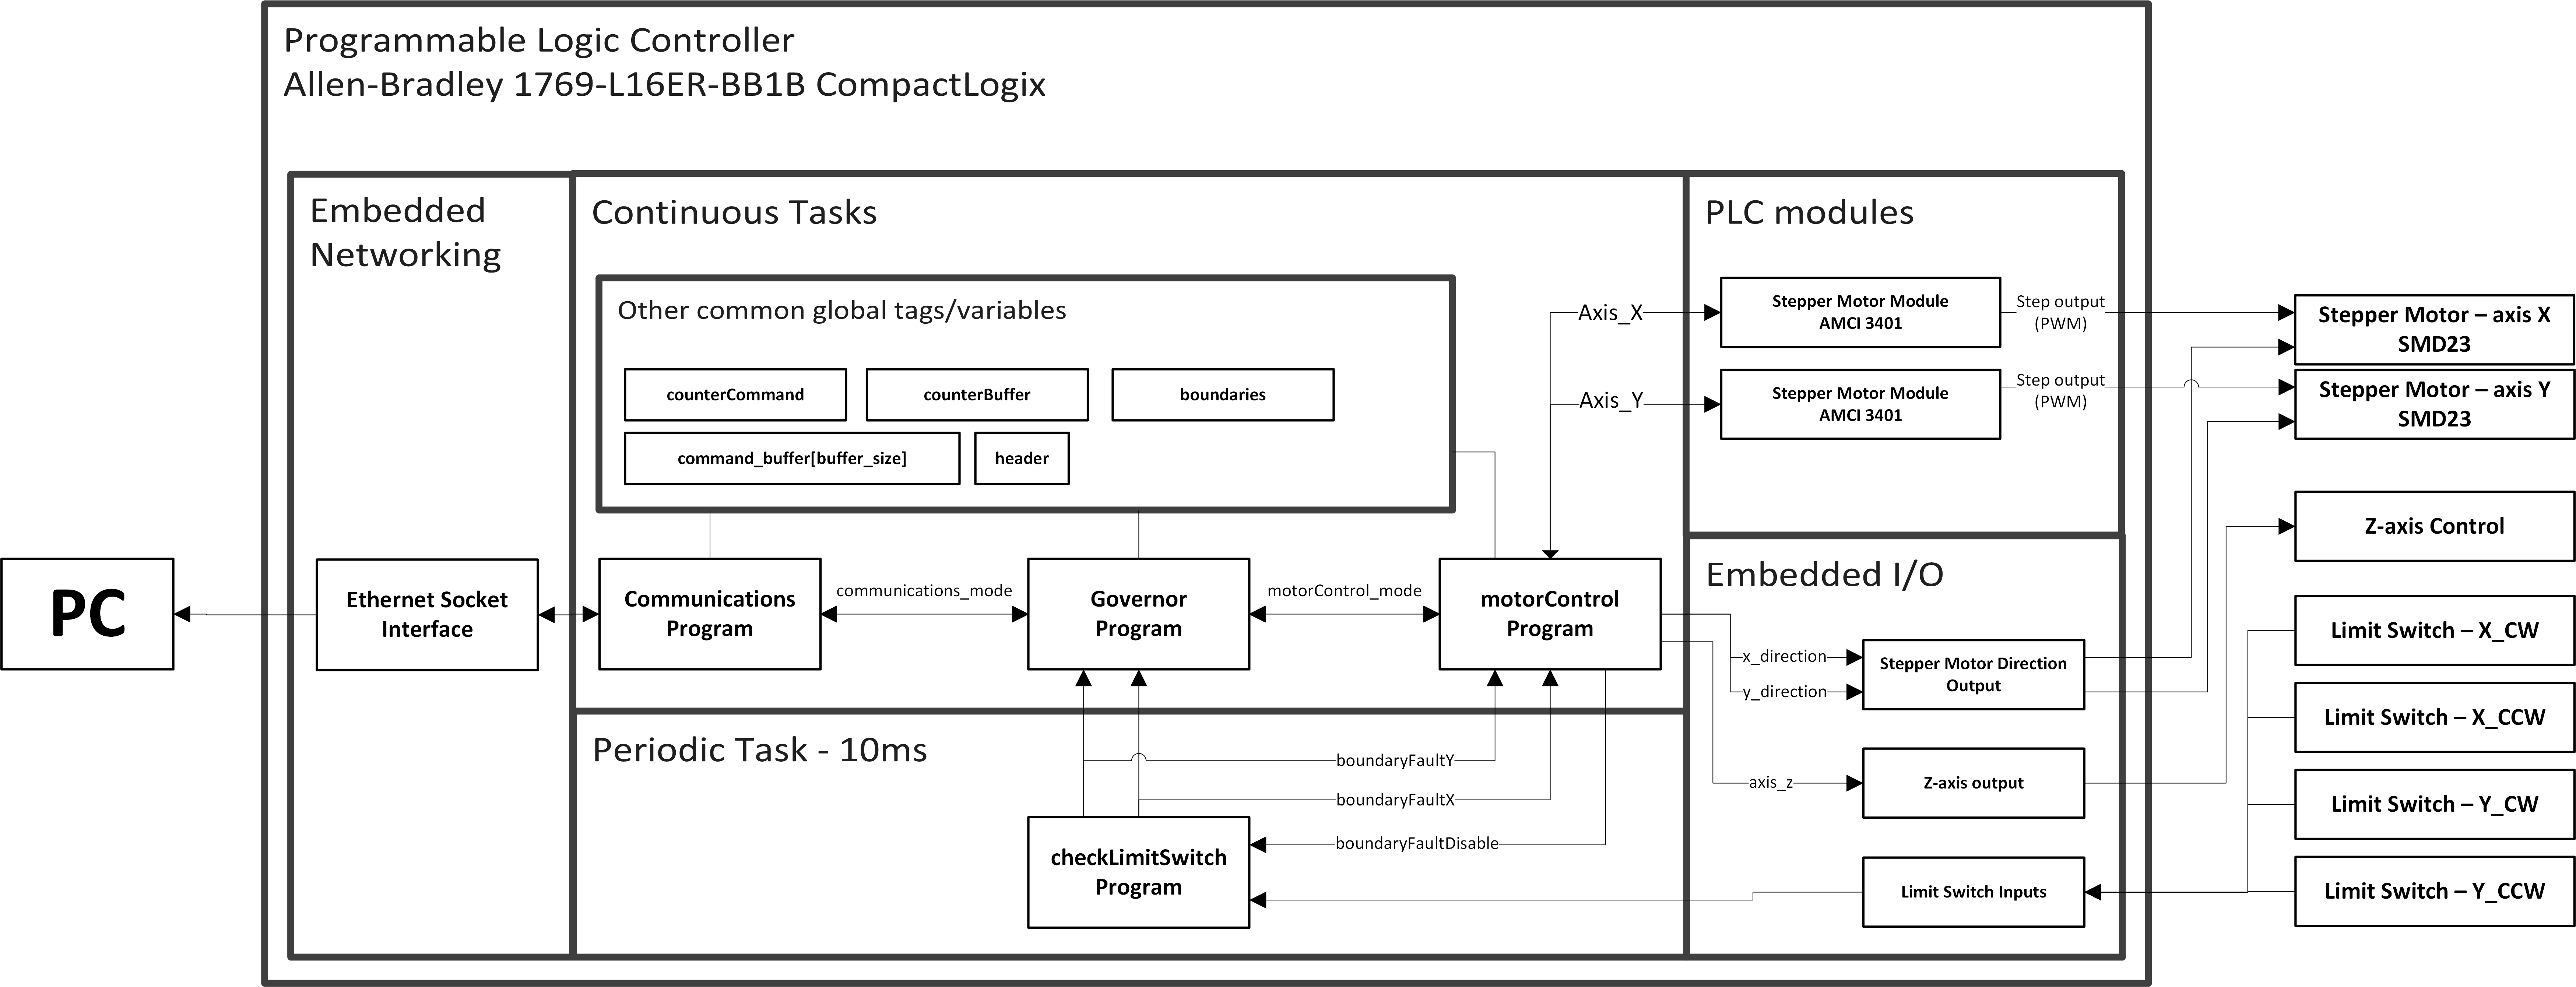
\includegraphics[width=\hsize]{figures/cncMachine/PLC_architecture}
		\captionof{figure}{The program and I/O architecture of the PLC}
		\label{fig:PLCarchitecture}
		\vspace*{\fill}
\end{landscape}


	\subsubsection{Programs}
		The programmable logic controller features four programs, shown visually in ~\ref{fig:PLCarchitecture}
	
		\begin{description}
			\item[Governor] \hfill \\
				The Governor state machine sets the overall state of the DoodleBot controller by interfacing with Communications and motorControl.
			\item[Communications] \hfill \\
				The Communications state machine is in charge of managing the UDP socket interface, all network communications and the populating of the command list.
			\item[motorControl] \hfill \\
				The motorControl state machine handles all stepper motor control and receives information from the checkLimitSwitch program.
			\item[checkLimitSwitch] \hfill \\
				The checkLimitSwitch program periodically monitors the limit switch input and triggers an emergency stop if the switches are triggered. It runs every 10ms.
		\end{description}
		
		\subsubsection{Intraprogram Interfaces and Global Data}
		The Governor program interfaces with the Communications and motorControl programs via the two global scope variables, \textit{motorControl\_mode} and \textit{communications\_mode} which act as intraprogram interfaces. On each state transition, the Governor sets these variables  to certain values, determining what state to move the other programs into. The other programs can then set these variables to different values, informing the Governor on their own state changes and status which the Governor then uses as state transition conditions. Table ~\ref{table:progaminterfaces} shows the possible values of the intraprogram interfaces. 
		
		\begin{table}[htbp!]
			\begin{tabular}{|c|l|l|l|}
				\hline
				Code & motorControl\_mode & communications\_mode & Set By \\ \hline
				00 & Wait & Wait & Governor \\ \hline
				10 & Initialize & Ready & Governor\\ \hline
				11 & Initialization complete & Header received & motorControl/communications \\ \hline
				20 & Operate commands & Buffer command list & Governor \\ \hline
				21 & All buffered commands complete & Buffering complete & motorControl/communications\\ \hline
				22 & N/A & Buffer full & communications\\ \hline
			\end{tabular}
			\caption{Codes for interface between Governor, Communications and motorControl programs}
			\label{table:progaminterfaces}
		\end{table}
	
		In addition to locally scoped variables, there are also several key global scope variables that are used by two or more program that determine the behaviour and input of the system. These are shown in Figure ~\ref{table:globalvariables}

	
		\begin{center}
			\begin{tabular}{|l|l|p{10cm}|}
				\hline
				Variable Name & Element & Description\\ \hline
			%Spill over is included as a 'row', so use 4 instead of 2 for multirow
				\multirow{4}{*}{counterCommand} & .counter & Index number of the command currently being operated on by motorControl (also, how many commands have been processed)\\ \cline{2-3}
					 & .pointer & Index of where the command referred to by counterCommand.counter resides in the commandBuffer array\\ \hline
				\multirow{4}{*}{counterBuffer} & .counter & Index number of the command currently being buffered by Communications (also, how many commands have been buffered)\\ \cline{2-3}
					 & .pointer & Index of where the command referred to by counterBuffer.counter resides in the commandBuffer array\\ \hline
				\multirow{8}{*}{commandBuffer[]} & .command\_no & Command number of what the current array element stores\\ \cline{2-3}
					& .type & Determines the command type. 0 is a 'draw' and 1 is a 'move'. \\ \cline{2-3}
					& .x\_speed & For 'draw' operations, determines the X target speed for this sample. For 'move' operations, determines the target position for X to move to. \\ \cline{2-3}
					& .y\_speed & For 'draw' operations, determines the Y target speed for this sample. For 'move' operations, determines the target position for Y to move to. \\ \hline
				\multirow{8}{*}{boundaries} & .X\_CW & The number of clockwise steps from the center until the boundary in the X positive direction\\ \cline{2-3}
					 & .X\_CCW & The number of clockwise steps from the center until the boundary in the X negative direction\\\cline{2-3}
					 & .Y\_CW & The number of clockwise steps from the center until the boundary in the Y negative direction\\ \cline{2-3}
					 & .Y\_CCW & The number of clockwise steps from the center until the boundary in the Y positive direction\\ \hline
				\multirow{6}{*}{header} & .delta\_time & Period of velocity profile samples\\ \cline{2-3}
					 & .no\_commands & Total number of commands to be received and executed on\\ \cline{2-3}
					 & .max\_accel\_x & Max acceleration in the X axis\\ \cline{2-3}
					 &  .max\_accel\_y & Max acceleration in the Y axis\\ \cline{2-3}
					 & .move\_speed\_x & Target speed for 'move' operations in the X axis\\ \cline{2-3}
					 & .move\_speed\_y & Target speed for 'move' operations in the Y axis\\ \hline
			\end{tabular}
			\captionof{table}{Important global scope variables used by multiple programs}
			\label{table:globalvariables}
		\end{center}

	\subsection{Governor}
		
		The Governor is a state machine that control the operation of the other programs in the DoodleBot system.
		
		\begin{description}
			\item[POWER\_ON] DoodleBot waits for the user to press one of the Y limit switches to state A to start initialization.
			\item[A\_Init] The DoodleBot checks the boundaries and centres itself on a 'home' position. After this is complete it progresses to state B.
			\item[B\_ready] The DoodleBot starts sending the 'ready' packet periodically to the PC, while waiting for a header to arrive. If a valid header arrives, it transitions to state C. If one of the Y limit switches are pressed, it returns to state A to run through the initialization routine once more.
			\item[C\_buffer] The DoodleBot begins requesting commands from the PC, filling the commandBuffer. When either the commandBuffer is full or all commands have been received, it progresses to state D.
			\item[D\_operating] The DoodleBot begins executing the commands in the commandBuffer. If there are still commands to received, it will continue to buffer when slots are freed up after being executed. After all commands have been processed the system returns to state B, ready for another header.
		\end{description}
		
		\begin{center}
				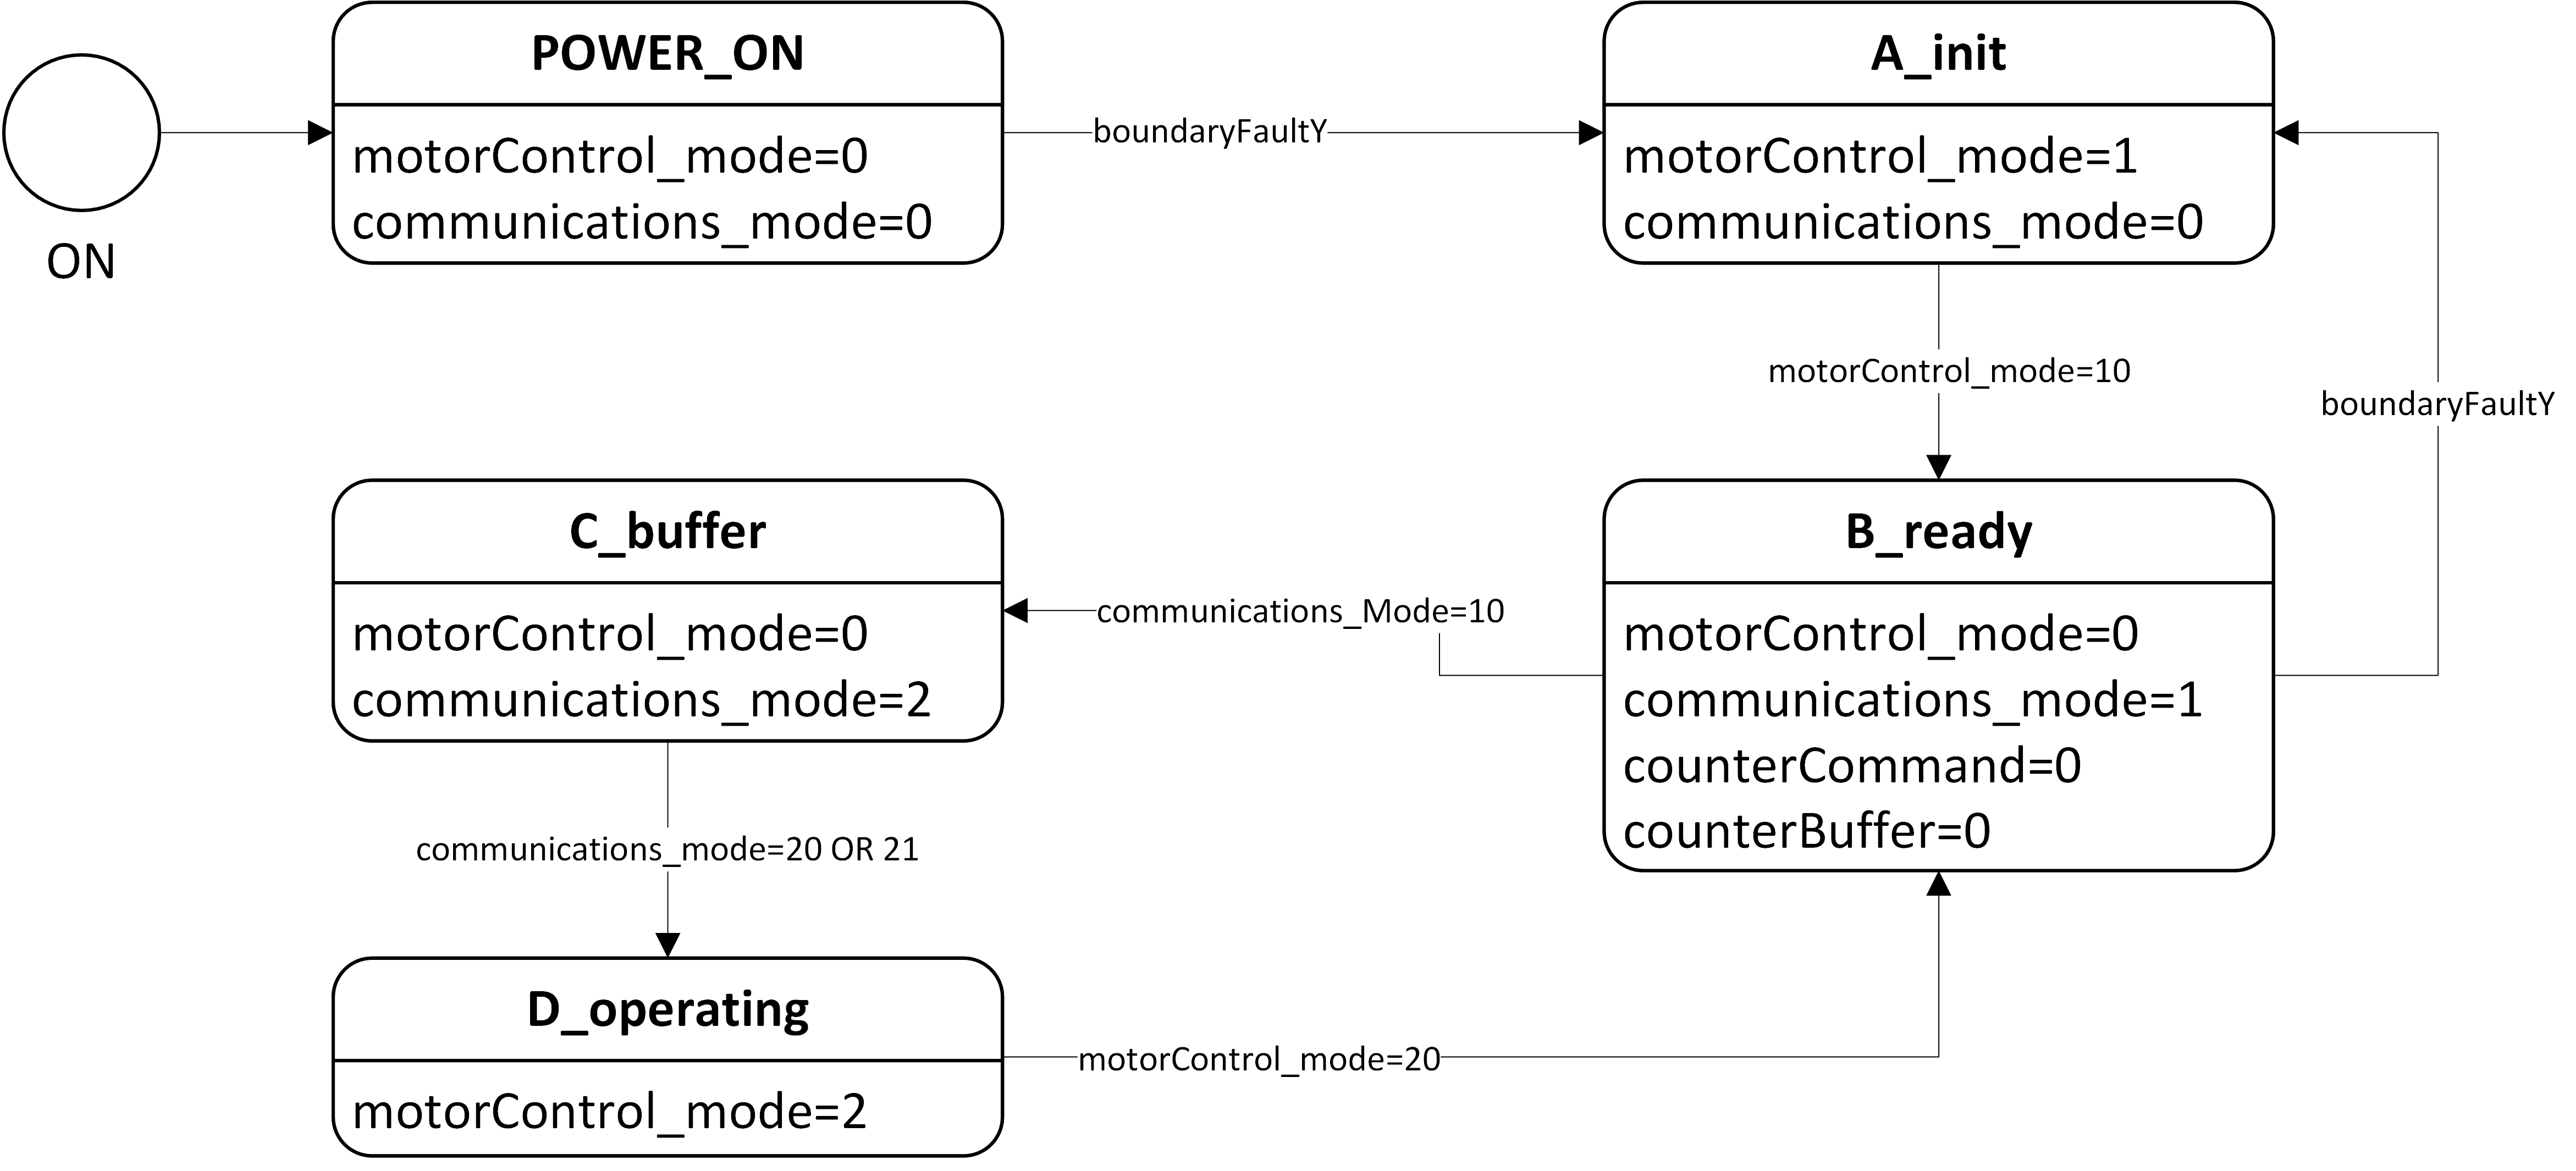
\includegraphics[width=\textwidth]{figures/cncMachine/governor}
				\captionof{figure}{The Governor State Machine}
				\label{fig:governor}
		\end{center}


\subsection{Communications}
	
	The communications program has the role of communicating with the PC to populate the commandBuffer with the output of the PCs optimization stage. Figure ~\ref{fig:communicationsStates} shows the operation of the program.

\subsection{motorControl}
	
	The motorControl Program's purpose is to control the electromechanical hardware via the AMCI 3401 Stepper Motor Modules and the PLC Embedded I/O. 
	
	Please see Appendix ~\ref{sec:PLC-flowcharts-motor} for more detail on how the motorControl Program functions and how the AMCI 3401 module works. A detailed flowchart of this program can be found in Figure ~\ref{fig:motorControlStates}.

	\subsubsection{Stepper Motor Direction Management}	
			Empirical observation of the AMCI 3401 modules in operation showed a significant delay (in the order of 2-3 seconds) between distinct commands. This delay was also present when switching between the Manual Move Clockwise and the Manual Move Counterclockwise commands. In contrast, changing the programmed speed while in either manual move state had negligible delay.
			
			This behaviour was a significant issue since the optimized velocity profiles require both axes to track the commands within the period of sampling (in the order of 30-150ms) to follow the required path and as such a 2-3 second delay would prevent proper operation.
			
			To overcome this problem, the DoodleBot controls the direction output via the PLC embedded DC output pins 0 and 1. Direction control is hence done  through code in the motorControl program rather than allow the AMCI 3401 modules to handle the task. To continue using Absolute Moves, this required extra code to keep track of the current position.
			
			Please see Appendix ~\ref{sec:PLC-flowcharts-pos} for more detail on how this part of the code works. A flowchart of this code can be found in Figure ~\ref{fig:Direction and Positional Tracking}.
			

\subsection{checkLimitSwitch}
	The checkLimitSwitch program is run in a Periodic Task of 10ms and monitors the four limit switches. Upon detecting a rising edge from one of these limit switches, it sets the appropriate boundaryFault value (boundaryFaultX for the X limit switches and boundaryFaultY for the Y limit switches).
	
	If the boundaryFaultDisable is NOT set, it will assume that unintended operation has occurred and an immediate stop command to the stepper motor modules halting all operation. If boundaryFaultDisable IS set then this operation does not happen (used in a situation where motorControl or the Governor are expecting a limit switch input. Eg, boundary checking or waiting for user to manually toggle the switch).